\scanpage{2}
% archive foliation: 1
\begin{center}\textbf{\Large COMMUNIQUE DE TOPOLOGIE STRUCTURALE}\end{center}

Le numéro 4 du bulletin est actuellement sous presse. Voici quelques exemples de ce que vous y trouverez.

\begin{minipage}[t]{.50\linewidth}
\textbf{Alan Holden} (New Jersey, USA) nous montre comment lier les anneaux polygonaux des tiges pour obtenir des formes polyédriques rigides. Exposant diverses possibilités à l'aide d'illustrations saisissantes de ses maquettes, il défie les lecteurs d'en trouver d'autres.

\textbf{David Georges Emmerich et Didier Aubry}, architectes à l'Ecole nationale supérieure des Beaux-Arts, Paris, étudient les empilements concentriques des polyèdres réguliers. De tels arrangements laissent des vides qui peuvent eux-mêmes être considérés comme étant des «polyèdres mixtes» dont les faces sont soit planes soit arrondies, bordées par des polygones réguliers (plans ou gauches).

\textbf{Michael Goldberg} (Washington DC, USA), mathématicien spécialisé dans l'étude des chaînons mécaniques, des rotors, des polyèdres et de leurs possibilités de juxtaposition, remanie son «autobiographie mathématique». A propos, un rotor est un ovale non circulaire capable de se mouvoir à l'intérieur d'un polygone régulier, entrant en contact avec tous ses côtés.

Reconsidérant ses études fort renommées sur les \unsure{zonaèdres|zonoèdres}, \textbf{Anton Hanegraaf} (Elst, Pays-Bas) nous invite à examiner un ensemble fascinant de vingt problèmes combinatoires.

Dans certaines positions, une structure normalement rigide, même isostatique, subit des mouvements finis ou infinitésimaux. \textbf{Ben Roth} (University of Wyoming, USA) formule une série de questions mathématiques concernant ces situations «particulières», et des fonctions d'énergie associées.

Du Form Studies Unit à Carleton University, Canada, \textbf{Gulzar Haider} nous parle des chaînons polyédriques et de leurs réseaux connexes, ainsi que de leurs applications architecturales.

\textbf{Tibor Tarnai}, du Hungarian Institute for Building Science, analyse, de son point de vue d'ingénieur, la rigidité des cylindres en treillis et réseaux munis de sommets sur la sphère.

On peut construire des polyèdres (et ensembles de polyèdres) ayant le même type de face, en fixant face à face des dodécaèdres réguliers. \textbf{Koji Miyazaki et Ichiro Takada} (Kobe University, Japon) nous présentent leur merveilleux travail magnifiquement illustré.
\end{minipage}\hfill
\begin{minipage}[t]{.46\linewidth}
\figure{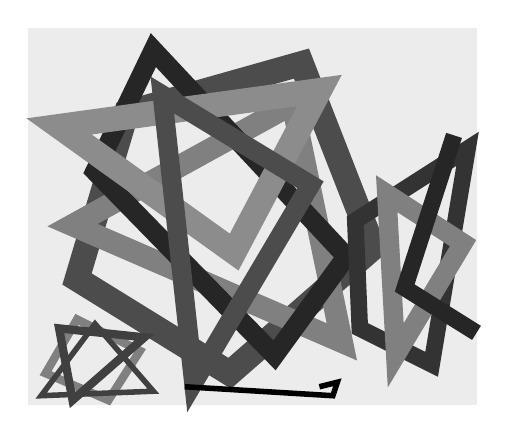
\begin{tikzpicture}[x=.57cm,y=.57cm]
\fill[gray!15] (0,0) rectangle (10,8.4);
\begin{scope}[line cap=butt,line join=miter]
\draw[black!70,line width=9pt] (1.1,2.8)--(2.2,6.5)--(6.1,7.6)--(7.7,3.5)--(4.5,.7)--cycle;
\draw[black!50,line width=8pt] (1.0,4.0)--(5.9,6.7)--(7.0,1.4)--cycle;
\draw[black!85,line width=7pt] (2.8,7.9)--(1.5,5.2)--(5.5,1.1)--(7.1,3.3)--cycle;
\draw[black!45,line width=9pt] (.7,6.2)--(4.6,3.4)--(6.5,7.0)--cycle;
\draw[black!70,line width=7pt] (3.0,6.9)--(6.3,4.9)--(3.7,.5)--cycle;
\draw[black!80,line width=6pt] (7.3,4.1)--(9.8,5.7)--(9.0,.9)--(7.4,1.7)--cycle;
\draw[black!50,line width=7pt] (8.0,4.7)--(9.7,3.6)--(8.2,1.1)--cycle;
\draw[black!85,line width=6pt] (9.5,6.0)--(8.4,2.6)--(10,1.6);
\draw[gray,line width=3pt] (.4,.7)--(1.1,1.9)--(2.5,1.2)--(1.8,.1)--cycle;
\draw[black!75,line width=2pt] (.3,.2)--(1.5,1.8)--(2.8,.3)--cycle;
\draw[black!75,line width=3pt] (.7,1.7)--(1.0,.1)--(2.6,1.5)--cycle;
\draw[line width=2pt] (3.5,.4)--(6.8,.2)--(6.9,.5)--(6.5,.4);
\end{scope}
\end{tikzpicture}}
% crop-candidate: scan 2

\figure{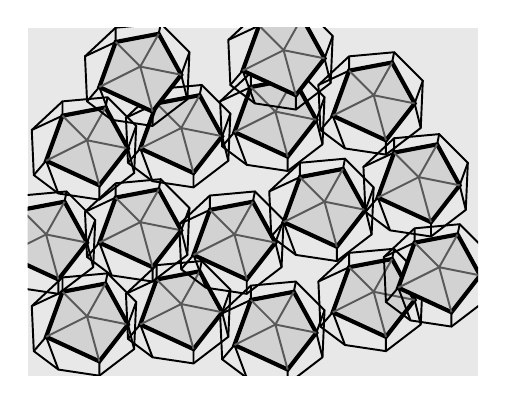
\begin{tikzpicture}[x=.52cm,y=.52cm,line width=.7pt]
\clip (0,0) rectangle (11,8.5);
\fill[gray!18] (0,0) rectangle (11,8.5);
\foreach \x/\y in {1.4/1.2,3.7/1.5,6/1,8.4/1.8,10/2.4,.4/3.2,2.7/3.5,5/3.2,7.2/4,9.5/4.6,1.4/5.5,3.7/5.8,6/6.2,8.4/6.6,2.7/7.3,6.2/7.7}{
\begin{scope}[shift={(\x,\y)}]
\fill[gray!35] (-.95,-.25)--(-.55,.85)--(.5,1.05)--(1.05,.05)--(.35,-.85)--cycle;
\draw (-1.25,-.6)--(-1.3,.5)--(-.55,1.2)--(.55,1.3)--(1.25,.6)--(1.2,-.55)--(.35,-1.2)--(-.65,-1.05)--cycle;
\draw[line width=1.5pt] (-.95,-.25)--(-.55,.85)--(.5,1.05)--(1.05,.05)--(.35,-.85)--cycle;
\draw (-1.25,-.6)--(-.95,-.25) (-1.3,.5)--(-.55,.85) (-.55,1.2)--(-.55,.85) (.55,1.3)--(.5,1.05) (1.25,.6)--(1.05,.05) (1.2,-.55)--(1.05,.05) (.35,-1.2)--(.35,-.85) (-.65,-1.05)--(-.95,-.25);
\draw[black!65] (-.55,.85)--(.05,.25)--(.5,1.05) (.05,.25)--(1.05,.05) (.05,.25)--(.35,-.85) (.05,.25)--(-.95,-.25);
\end{scope}}
\end{tikzpicture}}
% crop-candidate: scan 2
\end{minipage}

Topologie Structurale est un nouveau champ de recherche interdisciplinaire, faisant appel au talent de mathématiciens, architectes et ingénieurs, collaborant à sa réussite. Nous vous invitons à vous joindre aux efforts du groupe, et à communiquer vos idées en les publiant dans le bulletin. Si vous n'y êtes pas déjà abonné, pourquoi attendre? Faites-le dès aujourd'hui. Et si votre bibliothèque ne connaît pas encore Topologie Structurale, parlez-en au bibliothécaire sans plus tarder. Nous vous en serions très reconnaissants.
